\documentclass[aspectratio=169]{beamer} %handout
\usepackage{xcolor}

\definecolor{mznblue}{HTML}{1491eb}
\definecolor{mzngray}{HTML}{4a4a49}
\usecolortheme[named=mznblue]{structure}
\usecolortheme{seahorse}
\usecolortheme{orchid}
\setbeamercolor{palette primary}{use=structure,bg=mznblue,fg=white}
\setbeamertemplate{navigation symbols}{}
\setbeamertemplate{footline}{%
  % \begin{beamercolorbox}{section in head/foot}
  \vskip1pt%
  \scriptsize%
  \parbox[t][1em]{\paperwidth}{%
  \hspace*{10pt}\insertsection%
  \ifx\insertsubsection\empty\null\else~\texttt{>>}~\fi%
  \insertsubsection%
  \hfill%
  % \tiny%
  \insertframenumber%\,/\,\insertdocumentendpage%
  \hspace*{10pt}%
  }%
  \vskip4pt%
  % \end{beamercolorbox}%
}

\usepackage[english]{babel} %göra så att autogenererade saker blir på svenska
\usepackage[T1]{fontenc} %rendera åäö bättre
\usepackage[utf8]{inputenc} %använda utf-8
% \usepackage[parfill]{parskip} %gör så att styckena blir den "rätta" sorten
% \usepackage[indention=0.5cm]{caption}
\usepackage{mathtools}
% \usepackage{float}
% \usepackage{enumitem}
% \usepackage[margin=1in]{geometry}
\usepackage{helvet}
% \usepackage{courier}
\usepackage{graphicx}

% \newcommand\rebecka{asd}
% \ifdefined\rebecka yay \else nej \fi

\newif\iffast
\newcommand{\elnaturale}{\mathbb{N}}
\newcommand{\Oh}[1]{\mathcal{O} (#1)}
\usepackage{siunitx}
\sisetup{detect-all} % not math font or something

\iffast
\newcommand{\missingfigure}[1]{}
\newcommand{\todo}[1]{}
\usepackage{verbatim}
\newenvironment{tikzpicture}[1]{\comment}{\endcomment}
\else
% \usepackage{todonotes}
\usepackage{tikz}
\usetikzlibrary{arrows,positioning,calc,fit,arrows.meta,shadows}
\tikzset{big arrow/.style={-{Stealth[scale=1.4]}, shorten >=2pt}}
\tikzset{AST/.style = {
  minimum size=15pt,
  inner sep=0pt,
  every node/.style={circle, align=center},
  level distance=30pt,
}}
\usepackage{pgfplots}\pgfplotsset{compat=1.16}

\newcommand{\verticalline}[2]{\draw[#1]
($(current bounding box.north west)!#2!(current bounding box.north east)$)
--
($(current bounding box.south west)!#2!(current bounding box.south east)$)}
\fi

\usepackage{listings}
\usepackage{courier} % \texttt{...} gives thinner text and /\ displays OK

\newcommand\mznfont{\fontfamily{pcr}\selectfont}

\lstdefinestyle{mzn}{
  basicstyle=\mznfont,
  commentstyle=\color[rgb]{0.9,0.1,0.1},
  keywordstyle=\color[rgb]{0,0.5,0},
  keywordstyle=[2]\color{blue},
  stringstyle=\color{orange},
  tabsize=2,
  frame=none,
  % identifierstyle = \it,
  numbers=left,
  stepnumber=1,
  numberstyle=\tiny,
  numbersep=5pt,
  xleftmargin=0pt, % numbers will be in the margins!
  columns=fixed, % same width for all characters
  % columns=flexible,
  % columns=fullflexible,
  aboveskip={0pt},
  belowskip={0pt},
  showstringspaces=false,
  mathescape=true,
  breaklines=true,
  % prebreak=\raisebox{0ex}[0ex][0ex]{\ensuremath{\space\red{\swarrow}}},%\hookrightarrow
  % postbreak=\raisebox{0ex}[0ex][0ex]{\ensuremath{\textcolor{black}{\hookrightarrow\space}}},%\hookrightarrow
  % NOTE: beamer doesn't like color in postbreak.
  % https://tex.stackexchange.com/questions/586477/missing-number-treated-as-zero-within-beamer-and-lstcustom
  postbreak=\raisebox{0ex}[0ex][0ex]{\ensuremath{\hookrightarrow\space}},%\hookrightarrow
  breakatwhitespace=true,
  breakindent=0pt, % was: 20pt
  escapeinside={{<@}{@>}}
}

\lstdefinestyle{nonumbers} {
  numbers=none,
  xleftmargin=0pt,
}

\lstdefinelanguage{Mzn}
{
  morekeywords={
  %
  array, par, var, opt, constraint, solve, satisfy, minimize,
  maximize, output, include, let, in, set, of, if, then, else, endif,
  ann, annotation, bool, enum, float, int, string, where, function,
  predicate, true, false, not, assert, trace,
  % ???:
  any, list, op, record, test, tuple, type
  %
  },
  %
  keywords=[2]{
  %
  forall, sliding_sum, symmetry_breaking_constraint,
  implied_constraint, redundant_constraint, all_different,
  alldifferent, alldifferent_except_0, alldiff, element, circuit,
  subcircuit, dpath, card, bool2int, inter, count, regular, table, xor,
  exists, xorall, iffall, clause, intersect, diff, symdiff, subset,
  superset, concat, join, length, int_lt_reif, int_lin_eq_reif,
  bool_imply, array_bool_or, all_different_int, int_ne, at_least,
  at_most, exactly, count_eq, count_leq, count_geq, count_gt, nvalue,
  bin_packing, bin_packing_capa, bin_packing_load, diffn,
  global_cardinality, global_cardinality_closed, distribute,
  global_cardinality_low_up, global_cardinality_low_up_closed,
  inverse, cumulative, disjunctive, decreasing, increasing,
  strictly_decreasing, strictly_increasing, sort,
  arg_sort, value_precede, value_precede_chain, lex_less, lex_lesseq,
  lex_greater, lex_greatereq, lex2, strict_lex2, int_lin_eq, all_equal,
  bool_lin_eq, knapsack, partition_set, member, reverse, among, in_set,
  % from ???:
  abort, abs, acosh, array_intersect, array_union, array1d, array2d,
  array3d, array4d, array5d, array6d, asin, atan, bool2int, card,
  ceil, concat, cos, cosh, dom, dom_array, dom_size, fix, exp, floor,
  index_set, index_set_1of2, index_set_2of2, index_set_1of3,
  index_set_2of3, index_set_3of3, index_set_6of6, int2float, is_fixed,
  join, lb, lb_array, length, ln, log, log2, log10, min, max, pow,
  product, round, set2array, show, show_int, show_float, sin, sinh,
  sqrt, sum, tan, tanh, trace, ub, ub_array, xor, in, subset,
  superset, union, diff, symdiff, intersect, div, mod,
  % annotations:
  is_defined_var, output_var, var_is_introduced, defines_var,
  promise_total, bounds, domain, bool_search, int_search, seq_search,
  set_search, input_order, first_fail, anti_first_fail, smallest,
  largest, occurrence, most_constrained, max_regret, indomain_min,
  indomain_max, indomain_middle, indomain_median, indomain,
  indomain_random, indomain_split, indomain_reverse_split,
  indomain_interval, outdomain_max, outdomain_median, outdomain_min,
  outdomain_random, complete
  % 
  },
  sensitive=true,
  morecomment=[l]{\%},
  morestring=[b]",
  % morestring=[d]',
  moredelim=**[is][\color{Melon}]{@}{@},
}
%% Write "\begin{frame}[fragile]" for a slide using either of the
%% following two listing environments, which have unnumbered
%% respectively numbered lines:
\lstnewenvironment{mzn}[1][]{\lstset{language=Mzn,style=mzn,#1}}{}
\lstnewenvironment{mznno}[1][]{\lstset{language=Mzn,style=mzn,style=nonumbers,#1}}{}
\lstnewenvironment{mznnobreak}[1][]{\noindent\lstset{language=Mzn,style=mzn,style=nonumbers,#1}\minipage{\textwidth}}{\endminipage}
\BeforeBeginEnvironment{mznnobreak}{\par}
\AfterEndEnvironment{mznnobreak}{\par}

\lstnewenvironment{mznbreak}[1][]{\noindent\lstset{language=Mzn,style=mzn,#1}\minipage{\textwidth}}{\endminipage}
\BeforeBeginEnvironment{mznbreak}{\par}
\AfterEndEnvironment{mznbreak}{\par}
%% Inline a code snippet, without respectively with the comprehension bar (|):
\newcommand{\mzninline}[1]{\lstinline[{language=Mzn,style=mzn}]|#1|}
\newcommand{\mzninlinebar}[1]{\lstinline[{language=Mzn,style=mzn}]!#1!}

\newcommand{\mi}[1]{\mbox{\mzninline{#1}}}
\newcommand{\cpp}[1]{\mbox{\mznfont #1}}

\lstdefinestyle{diff}{
  morecomment=[f][\color{Green}]{+},
  morecomment=[f][\color{Red}]{-},
}
\lstnewenvironment{cppp}[1][]{\lstset{language={[11]C++},style=mzn,#1}}{}


\title{MiniZinc Linter}
\subtitle{Tool for Static Model Analysis}
\author{Erik Rimskog}
\institute{Uppsala University}
\date{}
% \logo{hej}

\AtBeginSection[]{
  \begin{frame}
    \frametitle{Outline}
    \tableofcontents[currentsection]
  \end{frame}
}
\AtBeginSubsection[]{
  \begin{frame}
    \frametitle{Outline}
    \tableofcontents[currentsection,currentsubsection]
  \end{frame}
}

\begin{document}

\begin{frame}[plain,noframenumbering]
  \titlepage
\end{frame}

\begin{frame}{Outline}
  \tableofcontents
\end{frame}

\section{MiniZinc}
% förklara MiniZinc
% introducera TSP
% MiniZinc + TSP = <3
% diagrammet över hela mzn
\begin{frame}{MiniZinc?}
  \begin{columns}[onlytextwidth]
    \column{0.2\textwidth}
    
\includegraphics[width=\textwidth]{mznlogo.png}
    % \vspace*{4cm}

    \column{0.75\textwidth}
    \begin{block}{What it is}
      Toolchain for solving combinatorial optimisation problems\pause{} using \emph{decision variables} ($x$) and \emph{constraints} ($x\neq4$).\pause{} It is solver independent.
    \end{block}
  \end{columns}

  \vspace{0.75cm}
  \pause
  \begin{block}{Travelling Salesman Problem}
    Find an order to visit $n \in \elnaturale^+$ cities in to minimise the total distance travelled.
  \end{block}
\end{frame}

% \begin{frame}{Travelling Salesman Problem}
%   \begin{block}{Problem Statement}
%     Find an order to visit $n \in \elnaturale^+$ cities in to minimise the total distance travelled.
%   \end{block}
%   \pause
%   \begin{center}
%     \begin{figure}[ht]
  \centering
  \begin{tikzpicture}[
    city/.style={draw, circle, minimum size=9mm},
    arr/.style={rectangle, minimum size=0.4cm},
    Arr/.style={-{Stealth}},
    ]
    \node (SLA) at (-3, -1) [city, label=above:Sala] {1};
    \node (HBY) at (2, 0) [city, label=above:Heby] {2};
    \node (MGA) at (5, -0.2) [city, label=above:Morgongåva] {3};
    \node (VIT) at (7.3, -1.4) [city, label=above:Vittinge] {4};

    \draw (SLA) edge[Arr,above, near start] node {20} (MGA)
          (MGA) edge[Arr,above] node {5} (HBY)
          (HBY) edge[Arr,above, near end] node {12} (VIT)
          (VIT) edge[Arr,below] node {26} (SLA);

    \node (A1) at (0, -3) [arr, label=north:1] {3};
    \node (A2) [arr, right=0 of A1, label=north:2] {4};
    \node (A3) [arr, right=0 of A2, label=north:3] {2};
    \node (A4) [arr, right=0 of A3, label=north:4] {1};
    \draw (A1.north west) -- (A4.north east) -- (A4.south east) -- (A1.south west) -- cycle;
    \draw (A1.north east) -- (A1.south east)
          (A2.north east) -- (A2.south east)
          (A3.north east) -- (A3.south east);

    \node [right=of A4] {$\sum = \SI{63}{km}$};
  \end{tikzpicture}
  \caption{Example instance of Travelling Salesman Problem with $n=4$ cities. The state is
    $\langle 3,4,2,1 \rangle$, which means that after city 1 is city 3 visited, after
    city 2 is city 4 visitied etc. The total distance travelled is \SI{63}{km}. Only the
    paths for the current route are shown.}%
  \label{fig:tsp}
\end{figure}

%   \end{center}
% \end{frame}

% \begin{frame}[fragile]{Travelling Salesman Problem Modelled}
% \begin{mznno}
% int: N = 4;                 % Amount of cities<@\pause@>
% set of int: Ns = 1..N;      % 1,2 .. N<@\pause@>
% array[Ns,Ns] of int: dist = % dist[1,2] = 15
%   [| 0,15,20,26
%    |15, 0, 5,12
%    |20, 5, 0, 5
%    |26,12, 5, 0|];<@\pause@>
% array[Ns] of var Ns: next;  % decision variables<@\pause@>
% include "globals.mzn";
% constraint circuit(next);   % connect as a loop<@\pause@>
% solve minimize sum(i in Ns) % minimize total distance
%                   (dist[i,next[i]]);<@\pause@>
% % solve satisfy;
% \end{mznno}
% \end{frame}

% \begin{frame}{MiniZinc Under the Hood}
%   \begin{block}{Solver}
%     Software that finds solutions to a model.
%   \end{block}
%   \pause
%   \begin{center}
%     \begin{tikzpicture}[
  grunka/.style={rectangle,draw,align=center},
  grej/.style={align=center,rectangle},
  solver/.style={minimum width=50pt},
  backend/.style={minimum width=65pt,minimum height=19pt},
  model/.style={minimum width=58pt,minimum height=17pt},
  shorten >=2pt,
  >=stealth'
  ]
  \node [grunka,model] (MZN) at (0, 0) {MiniZinc};
  \node [grunka,model] (DZN) at ($(MZN.center) + (0, -30pt)$) {Instance};
  \node [grunka] (FZN) [right=of MZN] {FlatZinc};
  \node [grunka,backend] (BKN) [right=of FZN] {fzn-gecode};
  \node [grunka,solver] (SLV) [right=of BKN] {Gecode};
  \node [grunka,backend,anchor=west] (BKN2) at ($(BKN.west) + (0,-30pt)$) {fzn-chuffed};
  \node [grunka,solver] (SLV2) at (SLV|-BKN2) {Chuffed};
  \node (ELI) [below=5pt of BKN2] {$\vphantom{\int^0}\smash[t]{\vdots}$};

  \node [above=23pt of MZN,grej,anchor=center] {High-level \\ Model};
  \node [above=23pt of FZN,grej,anchor=center] {Compiled \\ Model};
  \node [above=23pt of BKN,grej,anchor=center] {Backend};
  \node [above=23pt of SLV,grej,anchor=center] {Solver};

  \draw[->] (MZN) edge (FZN)
            (FZN) edge (BKN)
            (BKN) edge (SLV)
            (BKN2) edge (SLV2);
  \draw[->] (DZN.east) -- (FZN.south west);
  \draw[->] ($(FZN.east)!0.7!(BKN.west)$) |- (BKN2);
  \draw[dashed,->] ($(FZN.east)!0.7!(BKN.west)$) |- (BKN2.west|-ELI);

  \verticalline{dotted}{($(MZN.east)!0.5!(FZN.west)$)};
  \verticalline{dotted}{($(FZN.east)!0.5!(BKN.west)$)};
  \verticalline{dotted}{($(BKN.east)!0.5!(SLV.west)$)};
\end{tikzpicture}%

%   \end{center}
% \end{frame}

\section{Linter}
% förklara vad en linter är
% förklara några regler
% begränsingar?
\begin{frame}{Linter?}
  \begin{block}{Linter}
    A tool to perform static analysis on e.g.\@ source code.
    \pause
    \begin{itemize}
      \item Error-prone constructs
      \item Style
      \item Performance
      \item Simplify the code
    \end{itemize}
    \pause
    \textbf{Examples:} ESLint, HLint and Clippy.
  \end{block}

  \pause
  \begin{alertblock}{Not precise!}
    Many statements that can't be proven.
  \end{alertblock}
\end{frame}

\begin{frame}{Linter Rules}
  \begin{block}{Rule}
    A linter performs several checks, also called rules.
    Each rule can be disabled or enabled individually.
  \end{block}
\end{frame}

\begin{frame}{Example Execution}
  \texttt{\textcolor{green}{\bfseries\$}\;lzn model.mzn}\bigskip

  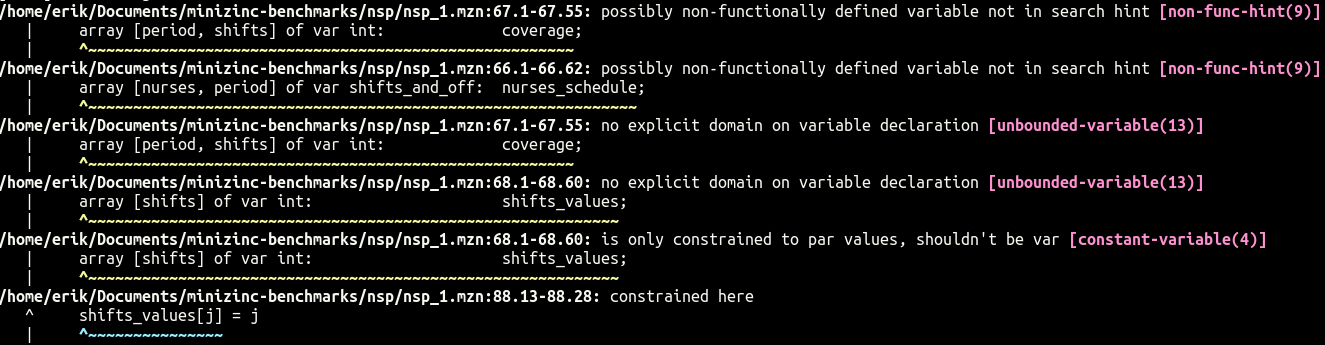
\includegraphics[width=\textwidth]{lznexample.png}
\end{frame}

\section{Rules}

\begin{frame}[fragile]{Unused Variables and Functions}
  \begin{block}{Motivation}
    Unused variables and functions don't contribute to the model and should be removed.\pause{}
    Being mentioned inside constraints or other used functions counts as usage.
  \end{block}

  \pause
  \begin{exampleblock}{Example}
  \begin{mznno}
var int: a;
var int: b; % unused
constraint a > 2;
solve satisfy;
  \end{mznno}
  \end{exampleblock}
\end{frame}

\begin{frame}[fragile]{Unused Variables and Functions Cont.}
  \begin{block}{Steps}
    \textbf{1.}~Find all variables and functions\quad
    \textbf{2.}~Calculate what depends on what\quad
    \textbf{3.}~Find all uses and recursively mark as used\quad
    \uncover<4->{\textbf{4.}~Simplify output}
  \end{block}

  \pause
  \begin{columns}[onlytextwidth]
    \column{0.6\textwidth}
    \begin{mznno}
int: K = 1;
int: N = 1;
int: M = let {int: J = 5} in J+N;
var 0..K: x;
function var int: f() = x+N;
solve minimize f();
    \end{mznno}
    \column{0.4\textwidth}
    \pause
    \begin{figure}[ht]
\centering
\smallskip%
\begin{tikzpicture}[
  every node/.style={draw, circle},
  -{Stealth[scale=1.2]},
  shorten >=2pt,
  used/.style={fill=green!50!white},
  contained/.style={fill=blue!35!white},
  ]
  \node (K) [used] at (0, 0) {\mi{K}};
  \node (x) [left=of K, used] {\mi{x}};
  \node (N) [above=of K, used] {\mi{N}};
  \node (f) [left=2 of N, used] {\mi{f}};
  \node (J) [below left=of f, contained] {\mi{J}};
  \node (M) [above=2 of J] {\mi{M}};

  \draw (x) edge (K)
        (f) edge (x)
        (f) edge (N)
        (M) edge (J)
        (M) edge (N);
\end{tikzpicture}%
\smallskip%
\caption{A dependency graph of an example model. An edge from a node to another means that
  the first node is directly depending on the other. For example is \mi{M} using \mi{N}.
  The green filled in nodes (\mi{f}, \mi{N}, \mi{x} and \mi{K}) are in use, and the blue
  filled node (\mi{J}) is ignored as it is contained inside of \mi{M}.}%
\label{fig:unused:graph}
\end{figure}

  \end{columns}
\end{frame}

\begin{frame}[fragile]{Missing Domain on Decision Variables}
  \begin{block}{Motivation}
    Decision variables should \alert{always} have tight domain to limit the amount of potential values.
  \end{block}

  \pause
  \begin{columns}[t,onlytextwidth]
    \column{0.47\textwidth}
  \begin{exampleblock}{Bad}
    \begin{mznno}
var int: a;
    \end{mznno}
  \end{exampleblock}

  \column{0.47\textwidth}
  \begin{exampleblock}{Good}
    \begin{mznno}
var 1..5: a;<@\pause@>
var int: b = a+1;
constraint b = a+1;
    \end{mznno}
  \end{exampleblock}
  \end{columns}
\end{frame}

\begin{frame}[fragile]{Missing Domain on Decision Variables Cont.}
  \begin{block}{Steps}
    \begin{enumerate}
      \item Find all decision variables
      \item Search constraints for equalities
    \end{enumerate}
  \end{block}

  \pause
  \begin{block}{$\land$-context}
    \begin{mznno}
constraint a=2;<@\pause@>
constraint a=2 /\ ...;<@\pause@>
constraint forall([a=2]);
    \end{mznno}
  \end{block}

  \pause
  \begin{alertblock}{Not always true}
    \begin{mznno}
constraint b=2 -> a=2;
    \end{mznno}
  \end{alertblock}
\end{frame}

\begin{frame}[fragile]{General Limitations}
  \begin{block}{Obfuscate}
    \begin{mznno}
constraint a=2 \/ false;
    \end{mznno}
  \end{block}

  \pause
  \begin{block}{Instance variables}
    No reliance on instance variables (parameters).\pause
    \begin{mznno}
int: A = 5;
array[1..A] of var int: xs;
constraint forall(i in 1..5)(xs[i] = ...)
    \end{mznno}
  \end{block}
\end{frame}

\section{Implementation}
% förklara AST
% återanvända parser
% förklara searchern
% regel-interfacet ??
\begin{frame}{Abstract Syntax Tree}
  \begin{columns}
    \column{0.67\textwidth}
  \begin{block}{Parser}
    Reads text and structures it into a data structure that can be processed, AST is a common one.
  \end{block}

  \pause
  \begin{block}{MiniZinc's parser was reused}
    \begin{itemize}
      \item Easier to maintain one than two
      \item Faster development
      \item Use existing functionality like the typechecker
    \end{itemize}
  \end{block}

  \column{0.27\textwidth}
  \pause
  \begin{center}
    
\includegraphics[width=0.9\textwidth]{cpp.png}
  \end{center}
  \end{columns}
\end{frame}

\begin{frame}[fragile,label=mznast]{MiniZinc AST}
  \begin{mznno}
   constraint x+42 = y;       var int: x = 1+1+1+1;
 \end{mznno}
 \hspace{2.75cm}$\Updownarrow$\hspace{6.3cm}$\Updownarrow$
 \bigskip
 \newif\ifshowastnumbers\showastnumbersfalse
 \newcounter{asdasd}

\begin{figure}[ht]
\centering
\begin{tikzpicture}[
label distance=-10pt,
every label/.style={blue},
lbl/.style={label=160:{\stepcounter{asdasd}\arabic{asdasd}}}
]
  \node at (0, 0) {\mi{constraint}} [sibling distance=60pt]
  child {node[lbl] {\cpp{BinOp} =}
    child {node[lbl] {\cpp{BinOp} +}
      child {node[lbl] (X) {\cpp{Id} ``x''}}
      child {node[lbl] {\cpp{IntLit} 42}}
    }
    child {node[lbl] {\cpp{Id} ``y''}}
  };

  \node (VX) at (6.5, 0) {\mi{var int: x}} [level 2/.style={sibling distance=140pt}, level 3/.style={sibling distance=65pt}]
  child {node[lbl] {\cpp{BinOp} +}
    child {node[lbl] {\cpp{BinOp} +}
      child {node[lbl] {\cpp{IntLit} 1}}
      child {node[lbl] {\cpp{IntLit} 1}}
    }
    child {node[label=177:{\stepcounter{asdasd}\arabic{asdasd}}] {\cpp{BinOp} +}
      child {node[lbl] {\cpp{IntLit} 1}}
      child {node[lbl] {\cpp{IntLit} 1}}
    }
  };

  \draw[-{Straight Barb[scale=1.3]},dashed] plot [smooth] coordinates {(X.south) ($(X.south) + (3, -0.3)$) ($(VX.west) + (-1.2, -0.5)$) (VX.west)};
\end{tikzpicture}
\caption{Illustration of two ASTs. The left one corresponds to \mi{constraint x+42=y},
  and the right one corresponds to \mi{var int: x=1+1+1+1}. The blue numbers are
  for referring to the nodes more easily and are not a part of the AST. The \mi{Id} at
  node 3 has a pointer to its declaration. \cpp{BinOp} is short for ``binary operation'',
  \cpp{Id} is short for ``identifier'' and lastly \cpp{IntLit} is short for ``integer
  literal''. These three are names of classes from MiniZinc.}%
\label{fig:ast:searcher}
\end{figure}

\end{frame}

\begin{frame}{AST Searcher}
  \begin{block}{Visitors}
    Using existing visitors would have been \alert{verbose}. They are better for processing the whole tree.
  \end{block}

  \pause
  \begin{block}{Searcher}
    Find locations in an AST from a path specification.\pause{}
    \texttt{>} means directly under, \texttt{>{}>} means under at any depth.
    \begin{itemize}
      \item \texttt{+ >{}> int}\pause
      \item \texttt{= > id}\pause
      \item \texttt{let > = >{}> + > id}
    \end{itemize}
  \end{block}
\end{frame}

\againframe{mznast} %TODO: animate?

\begin{frame}{Overview}
  \begin{columns}
    \column{0.67\textwidth}
    \begin{center}
      \begin{figure}[ht]
\centering
\smallskip%
\begin{tikzpicture}[
  blackrekt/.style={draw, rectangle},
  number/.style={auto,draw,circle,solid,inner sep=1pt,outer sep=3pt, node font=\scriptsize, very thin},
]
  \node (LE) at (0, 0) {\cpp{LintEnv}};
  \node (IP) [blackrekt, below=0.2 of LE.south west, anchor=north west] {Include paths};
  \node (AST) [blackrekt, right=0.2 of IP] {AST};
  \node (RES) [double copy shadow={shadow xshift=4pt, shadow yshift=0}, fill=white, blackrekt, below=0.2 of IP.south west, anchor=north west] {\cpp{LintResult}};
  \node (BOX) [fit=(LE) (IP) (AST) (RES), blackrekt] {};

  \newcommand{\lintrule}[2]{
    \node (#1) at #2 {\cpp{LintRule}};
    \draw[fill=white] (#1.north west) +(0, 0.5) -| ($(#1.north west)!0.3!(#1.north east)$)
    -- ($(#1.north west)!0.7!(#1.north east)$) |- ($(#1.north east) + (0, 0.5)$)
    -- (#1.south east) -- (#1.south west) -- cycle;
  }
  \foreach \y in {-4.2, -4.1, -4} \lintrule{LR1}{(-\y, \y)};
  \node (PR1) at (4, -4) {\cpp{LintRule}};
  \draw[big arrow, shorten >=8pt] (BOX) edge[out=0, in=90] node [number, near start] {1} (LR1);
  \draw[big arrow, dashed] (LR1) edge[out=180,
  in=-90] node [number] {2} ($(BOX.south) + (0.5, 0)$);

  \node (PRT) [rectangle, align=left, draw=black, line width=1mm, rounded corners, inner sep=2mm] at (-3, -3.6) {\texttt{\textbf{\Large >\_}} \\ Stdout printer};
  \draw [big arrow] (RES) edge[in=90,out=180,looseness=1.3] node [number] {3} (PRT);

\end{tikzpicture}%
\smallskip%
\caption{Illustration for the main execution of the linter. The \cpp{LintEnv} is given as
  an argument to each \cpp{LintRule} (1). Each rule will analyse the AST and write its
  results back to a list inside \cpp{LintEnv} (2). When all rules have been processed, is
  the list of all results given to a function that will output them back to the user
  (3).}%
\label{fig:overview}
\end{figure}

    \end{center}

    \pause
    \column{0.3\textwidth}
    \begin{enumerate}
      \item Each rule reads the AST from the environment\pause
      \item They write back results\pause
      \item The results are displayed in some way
    \end{enumerate}
  \end{columns}
\end{frame}

% \section{Results}
% förklara nurses
% minizinc benchmarks
% \section{Future Work}
% \begin{frame}{Future Work}
%   \begin{itemize}
%     \item Commandline interface\pause
%     \item Config language
%   \end{itemize}
% \end{frame}

\section{Summary}
\begin{frame}{Summary}
  \begin{itemize}
    \item MiniZinc is a modelling language that can be used on different solvers.
    \item Decision variables are unknows and constraints constrain them.
    \item A linter for static analysis of models was created.
    \item Some things are impossible to deduce.
    \item Written in C++.
    \item The MiniZinc parser was reused.
    \item An AST searcher searches for locations of interest in models.
  \end{itemize}
\end{frame}

\end{document}

